%=============================================================
% Ricardo Costa, November, 2024
%=============================================================
% - Article chapter template
% - In this chapter format, an abstract and keywords appear on the first page and the sections start
% on the next page
% - A table of contents and list of figures and tables can be generated for this chapter individually,
% and for that uncomment the commands \minitoc, \minilof, and \minilot below
% - If any of the above commands are used, also uncommented the command \newpage below for a
% page break (in that case, sections start on the next available page)
% - Sections in this chapter are also included in different files for the sake of organization (especially
% useful for large documents) but a single file with all the sections can also be used
% - All the sections, figures, tables, and any other material used in this chapter are in folder include/
% but any other structure can be used providing the appropriate paths to the commands
% - A bibliography can be generated for this chapter individually, and for that uncomment the last
% commands at the end of this file and provide the path to the bibliography file
% - The last three commands are suffixed with "chapi", which is an identifier for the bibliography
% included in the current chapter, in that case chap1
% - Replace the suffix "chapii" with "chapiii", "chapiv", "chapv", "chapvi", etc. according to the current
% chapter number and for each chapter you want to generate an individual bibliography (for instance,
% in "chap6.tex" replace the suffix "chapii" with "chapvi" in the last three commands)
% - If individual bibliographies are used for each chapter, comment the last commands in the main
% file to not generate a global bibliography (it is recommended to have either a global bibliography
% or individual bibliographies for each chapter)
% - Consider using the prefix "chapX:" (replace X with the chapter number) in each label you create
% for the sections, figures, tables, equations, and bibliography to avoid duplicate references between
% chapters (for instance, \label{chap2:some_figure}, @article{chap2:some_paper}, etc.)
%=============================================================

% chapter title
\chapter{Very high-order accurate finite volume scheme for the convection-diffusion equation}

% do not comment or modify
\afterpage{\global\bodystyleheadertrue}

% leave this uncommented to cite the associated article as a footnote
\blfootnote{This chapter was adapted from R. Costa, J.M. N\'obrega, S. Clain, G.J. Machado, and R. Loub\`ere, Very high-order accurate finite volume scheme for the convection-diffusion equation with general boundary conditions on arbitrary curved domains, Int. J. Numer. Meth. Engrg. 117(2) (2019) 188--220, DOI: https://doi.org/10.1002/nme.5953}

% chapter abstract
\begin{chapterabstract}
Obtaining very high-order accurate solutions in curved domains is a challenging task as the accuracy of conventional discretization methods, usually developed for polygonal domains, dramatically reduce without an appropriate treatment of boundary conditions.
The classical techniques to preserve the optimal convergence order are found in the context of finite element and finite volume methods, which often rely on curved mesh elements to fit the associated curved boundary.
Such techniques demand sophisticated meshing algorithms, cumbersome quadrature rules for integration, and complex non-linear transformations to map the curved mesh elements onto the reference polygonal ones.
In this regard, the Reconstruction for Off-site Data method provides very high-order accurate polynomial reconstructions on arbitrary smooth curved boundaries, enabling the integration of the governing equations in polygonal mesh elements and, therefore, avoiding the use of complex integration quadrature rules or non-linear transformations.
The method was initially introduced for Dirichlet boundary conditions, and the present work proposes an extension for general boundary conditions, which represents an important advance for real context applications.
A generic framework to compute polynomial reconstructions is also developed based on the least-squares method, which handles general constraints and further improves the algorithm.
The proposed methods are applied to solve the convection-diffusion equation with a finite volume discretization in general unstructured meshes.
A comprehensive numerical benchmark is provided to verify and assess the accuracy, convergence orders, robustness, and efficiency of the method.
The results prove that the method is capable of fulfilling boundary conditions appropriately on arbitrary smooth curved boundaries, and a very high-order of convergence is effectively achieved.
\end{chapterabstract}

% chapter keywords
\begin{chapterkeywords}
Very high-order accurate finite volume scheme, arbitrary smooth curved boundaries, general boundary conditions, polynomial reconstructions, least-squares method, reconstruction for off-site data method, convection-diffusion equation
\end{chapterkeywords}

% leave this uncommented for an individual chapter table of contents
%\minitoc
% leave this uncommented for an individual chapter list of figures
%\minilof
% leave this uncommented for an individual chapter list of tables
%\minilot
% leave this uncommented if any of the above commands are used
%\newpage

% include section files
\section{Introduction}
\label{chap2:sec:introduction}

The treatment of ever-increasing complexity problems in engineering has only been possible due to the capabilities of modern-day computational methods and high-performance computers.
In what concerns to the numerical modelling, computational efficiency is usually determined based on the computational effort necessary to obtain a certain level of solution accuracy, leading to a trade-off between the convergence order of the method and the mesh characteristic size.
In the absence of shocks or irregularities, increasing the convergence order is more efficient concerning computational resources than mesh refinement.
However, obtaining very high-order accurate approximations is still a challenging task, and many developments in that field are to be made.

The majority of the very high-order accurate methods (more than the second-order) are specifically designed for polygonal (or polyhedral) domains and, usually, numerical difficulties in obtaining the optimal convergence order arise when handling boundary conditions prescribed on curved boundaries.
For a short literature review on the topic, the reader is referred to the introduction section in R. Costa et al., 2018~\cite{chap2:2018costa1}, which is summarized in the following.
The classical approach to handle boundary conditions on curved boundaries is based on the isoparametric element method~\cite{chap2:2016lehrenfeld,chap2:2017lehrenfeld}, which requires, on one side, the introduction of curved mesh elements and, on the other side, non-linear transformations to map the local curved mesh elements onto the reference polygonal ones.
An alternative approach, dedicated to the finite volume method, was initially proposed by C. Ollivier-Gooch et al., 2002~\cite{chap2:2002ollivier}.
The technique does not require non-linear transformations, but the main shortcoming remains, in particular, the meshing algorithm to generate curved mesh elements fitting curved boundaries in addition to the high-order accurate quadrature rules for numerical integration on non-polygonal mesh elements.
As a consequence, handling arbitrary two- or three-dimensional curved elements turns out to be a cumbersome task, which results in significant computational costs~\cite{chap2:2009geuziane,chap2:2014wang,chap2:2015moxey}.

R. Costa et al., 2018~\cite{chap2:2018costa1}, introduced a new approach in the finite volume context, the reconstruction for off-site data method (shortened to ROD method), which is capable of handling boundary conditions on arbitrary smooth curved boundaries with a very high-order of convergence.
The novelty of the method is to use only polygonal mesh elements, overcoming the mismatch between the mesh boundary and the domain boundary.
The method enforces the prescribed boundary conditions using polynomial reconstructions in the vicinity of the boundary, which are computed based on the constrained least-squares method.
Moreover, the governing equations are integrated on polygonal mesh elements and, consequently, the numerical heat fluxes are determined solely on the boundaries of the polygonal cells.
Therefore, no sophisticated meshing algorithms for curved mesh elements are required, nor non-linear transformations, nor cumbersome quadrature rules for integration in the curved elements.
There are very few methods capable of handling curved domains with polygonal meshes, and most of them are limited to the first- or second-order of convergence.
Recently an extension of the immersed boundary method to the fourth-order of convergence has been proposed in the framework of the Fourier spectral method~\cite{chap2:2016stein,chap2:2017stein}, which is able of handling arbitrary smooth curved domains.

The ROD method was initially developed only for the steady-state two-dimensional convection-diffusion problem with Dirichlet boundary conditions.
In the present work, essential developments are introduced to the method, namely, the handling of Neumann and Robin boundary conditions, which represents a fundamental advance for real context applications.
Moreover, the development of a generic framework to compute polynomial reconstructions based on the least-squares method allows the handling of general constraints and improves the algorithm.

The remaining sections of the chapter are organized as follows.
Section~2 presents the model, the mesh, and the basic assumptions and notations.
Section~3 introduces the generic framework to compute polynomial reconstructions based on the least-squares method.
Section~4 is dedicated to the ROD method based on the previously introduced polynomial reconstructions and the Dirichlet, Neumann, and Robin boundary conditions on curved boundaries are addressed.
Section~5 presents the very high-order accurate finite volume scheme based on the polynomial reconstructions and the ROD method.
Section~6 provides a comprehensive numerical benchmark test suite to verify and assess the proposed method.
The chapter is completed in Section~7 with the conclusions and some perspectives for future work.

% end of file

\section{Mathematical formulation}
\label{chap2:sec:mathematical_formulation}

The steady-state convection-diffusion problem is addressed in two dimensions and formulated with the Cartesian coordinate system considering $\bm{x}\coloneqq\left(x,y\right)$.
Let $\Omega$ be an open bounded domain of $\mathbb{R}^{2}$ with boundary $\Gamma$, partitioned into three non-overlapping and possibly empty subsets, $\Gamma^{\textrm{D}}$, $\Gamma^{\textrm{N}}$, and $\Gamma^{\textrm{R}}$, such that $\Gamma=\Gamma^{\textrm{D}}\cup\Gamma^{\textrm{N}}\cup\Gamma^{\textrm{R}}$.
The boundary and the interface are regular Jordan curves, that is, simple and closed curves, and admit a known local parameterization.
Vector $\bm{n}=\left(n_{x},n_{y}\right)\coloneqq\left(n_{x}\left(\bm{x}\right),n_{y}\left(\bm{x}\right)\right)$ stands for the outward unit normal vector to $\Gamma$ at point $\bm{x}$ on the boundary (see Figure~\ref{chap2:fig:mathematical_formulation_domain}).

\begin{figure}[!htb]
\centering
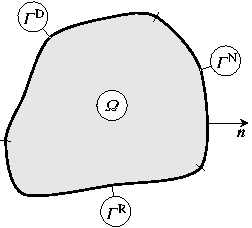
\includegraphics[width=4.5cm]{chap2/include/tikz/curved_domain}
\caption{Example of arbitrary curved domain with boundary subsets and outward unit normal vector.}
\label{chap2:fig:mathematical_formulation_domain}
\end{figure}

\subsection{Convection-diffusion model}
\label{chap2:subsec:mathematical_formulation_convection_diffusion_model}

The governing equation for temperature function $\phi\coloneqq\phi\left(\bm{x}\right)$ is given as
\begin{equation}
\nabla\cdot\left(\bm{u}\phi-\kappa\nabla\phi\right)=f,\quad\text{ in }\Omega,
\label{chap2:eq:mathematical_formulation_convdiff}
\end{equation}
where $\bm{u}\coloneqq\left(u_{x},u_{y}\right)\coloneqq\left(u_{x}\left(\bm{x}\right),u_{y}\left(\bm{x}\right)\right)$ is the velocity vector function multiplied by the heat capacity and density of the associated material, $\kappa\coloneqq\kappa\left(\bm{x}\right)$ is the thermal conductivity function, and $f\coloneqq f\left(\bm{x}\right)$ is the heat source function (a negative value implies a heat sink).
All functions are assumed to be regular and bounded in the domain.
To complete Equation~\cref{chap2:eq:mathematical_formulation_convdiff}, boundary subsets $\Gamma^{\textrm{D}}$, $\Gamma^{\textrm{N}}$, and $\Gamma^{\textrm{R}}$ are prescribed with the following boundary conditions:
\begin{itemize}
\item On boundary subset $\Gamma^{\textrm{D}}$, a Dirichlet boundary condition is prescribed, given as
\begin{equation}
\label{chap2:eq:mathematical_formulation_dirichlet}
\phi=g^{\textrm{D}},\quad\text{on }\Gamma^{\textrm{D}},
\end{equation}
where $g^{\textrm{D}}\coloneqq g^{\textrm{D}}\left(\bm{x}\right)$ is a given regular function.
\item On boundary subset $\Gamma^{\textrm{N}}$, a Neumann boundary condition is prescribed, given as
\begin{equation}
\label{chap2:eq:mathematical_formulation_neumann}
-\kappa\nabla\phi\cdot\bm{n}=g^{\textrm{N}},\quad\text{on }\Gamma^{\textrm{N}},
\end{equation}
where $g^{\textrm{N}}\coloneqq g^{\textrm{N}}\left(\bm{x}\right)$ is a given regular function.
\item On boundary subset $\Gamma^{\textrm{R}}$, a Robin boundary condition is prescribed, given as
\begin{equation}
\label{chap2:eq:mathematical_formulation_robin}
\alpha^{\textrm{R}}\phi+\beta^{\textrm{R}}\nabla\phi\cdot\bm{n}=g^{\textrm{R}},\quad\text{on }\Gamma^{\textrm{R}},
\end{equation}
where $g^{\textrm{R}}\coloneqq g^{\textrm{R}}\left(\bm{x}\right)$, $\alpha^{\textrm{R}}\coloneqq\alpha^{\textrm{R}}\left(\bm{x}\right)$, and $\beta^{\textrm{R}}\coloneqq\beta^{\textrm{R}}\left(\bm{x}\right)$ are given regular functions.
For instance, if $\alpha^{\textrm{R}}\left(\bm{x}\right)\coloneqq\bm{u}\left(\bm{x}\right)\cdot\bm{n}\left(\bm{x}\right)$ and $\beta^{\textrm{R}}\left(\bm{x}\right)\coloneqq-\kappa\left(\bm{x}\right)$, then the Robin boundary condition represents a total heat flux boundary condition.
The Robin boundary condition can also be used to prescribe mixed boundary conditions of Dirichlet and Neumann types.
\end{itemize}

\subsection{Polygonal meshes}
\label{chap2:subsec:mathematical_formulation_polygonal_meshes}

A general polygonal mesh denoted as $\mathcal{M}$ discretizes the subdomain $\Omega$ and consists of $n$ non-overlapping convex polygonal cells (triangles, quadrangles, etc.).
Cells are denoted as $c_{i}$ with $i\in\mathcal{I}=\lbrace 1,\ldots,n\rbrace$.
Inner edges are denoted as $e_{ij}$ with $j\neq i$ and $i,j\in\mathcal{I}$ and correspond to the edges shared between neighbour cells $c_{i}$ and $c_{j}$ and, therefore, $e_{ij}=c_{i}\cap c_{j}$.
Boundary edges are denoted as $e_{iF}$ with $i\in\mathcal{I}^{F}$, $F\in\lbrace\textrm{D},\textrm{N},\textrm{R}\rbrace$, and correspond to the edges of cells $c_{i}$ approximating boundary subsets $\Gamma^{F}$ (for the sake of simplicity, each cell has at most one boundary edge).
Subset $\mathcal{I}^{F}\subset\mathcal{I}$ gathers the indices and $n^{F}$ is the number of the cells with a boundary edge approximating boundary subset $\Gamma^{F}$.
The vertices of the boundary edges fall on the curves of the associated boundary subsets.

Table~\ref{chap2:tab:mathematical_formulation_notations} introduces the geometric properties for the cells and edges and Figures~\ref{chap2:fig:mathematical_formulation_notations} provides a schematic representation.
Notice that inner edge $e_{ij}$ is also denoted as $e_{ji}$ and, therefore, reference and quadrature points are the same, that is, $\bm{m}_{ij}=\bm{m}_{ji}$ and $\bm{q}_{ij,r}=\bm{q}_{ji,r}$, whereas outward unit normal vectors are antisymmetric, that is, $\bm{s}_{ij}=-\bm{s}_{ji}$.

\begin{table}[!htb]
\centering
\caption{Notation and geometric properties for the cells and edges.}
\label{chap2:tab:mathematical_formulation_notations}
\resizeboxlarger{
\begin{tabular}{@{}lllll@{}}
\toprule
Mesh elements & Notation & Properties & Definition & Choice\\
\midrule
\multirow{5}{*}{Cells} & \multirow{5}{*}{$c_{i}$} & $\partial c_{i}$ & Boundary & \\
& & $\vert c_{i}\vert$ & Area & \\
& & $\bm{m}_{i}=\left(m_{i,x},m_{i,y}\right)$ & Reference point (can be any point in $c_{i}$) & Centroid \\
& & $\bm{q}_{i,q}=\left(q_{i,q,x},q_{i,q,y}\right)$ & Quadrature points, $q=1,\ldots,Q$ & Gaussian \\
& & $\mathcal{N}_{i}$ & Indices of the adjacent cells and boundary subset & \\
\midrule
\multirow{4}{*}{Inner edges} & \multirow{4}{*}{$e_{ij}$} & $\vert e_{ij}\vert$ & Length & \\
& & $\bm{m}_{ij}=\left(m_{ij,x},m_{ij,y}\right)$ & Reference point (can be any point on $e_{ij}$) & Midpoint\\
& & $\bm{q}_{ij,r}=\left(q_{ij,r,x},q_{ij,r,y}\right)$ & Quadrature points, $r=1,\ldots,R$ & Gaussian \\
& & $\bm{s}_{ij}=\left(s_{ij,x},s_{ij,y}\right)$ & Outward unit normal vector from cell $c_{i}$ to cell $c_{j}$ & \\
\midrule
\multirow{4}{*}{Boundary edges} & \multirow{4}{*}{$e_{iF}$} & $\vert e_{iF}\vert$ & Length & \\
& & $\bm{m}_{iF}=\left(m_{iF,x},m_{iF,y}\right)$ & Reference point (can be any point on $e_{iF}$) & Midpoint\\
& & $\bm{q}_{iF,r}=\left(q_{iF,r,x},q_{iF,r,y}\right)$ & Quadrature points, $r=1,\ldots,R$ & Gaussian \\
& & $\bm{s}_{iF}=\left(s_{iF,x},s_{iF,y}\right)$ & Outward unit normal vector from $c_{i}$ & \\
\bottomrule
\end{tabular}
}
\end{table}
\vspace{1.0cm}

\begin{figure}[!htb]
\centering
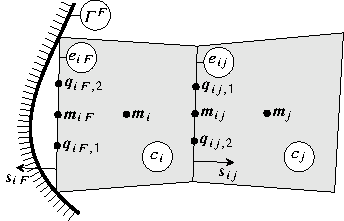
\includegraphics[height=4.5cm]{chap2/include/tikz/mesh2d_boundary}
\caption{Notation and geometric properties for the cells and edges.}
\label{chap2:fig:mathematical_formulation_notations}
\end{figure}

In the scope of work, keywords physical and computational distinguish the real domain from the discretized domain, respectively, and in this way, the following definitions are introduced:
\begin{itemize}
\item The computational domain, denoted as $\Omega_{\Delta}$, gathers all the cells and stands for a representative approximation of physical domain $\Omega$, given as
\begin{equation}
\Omega_{\Delta}=\bigcup_{i\in\mathcal{I}}c_{i}.
\end{equation}

\item The computational boundary, denoted as $\Gamma_{\Delta}$, gathers all the boundary edges and stands for a representative approximation of physical boundary $\Gamma$, given as
\begin{equation}
\Gamma_{\Delta}=\bigcup_{i\in\mathcal{I}^{F},F\in\lbrace\textrm{D},\textrm{N},\textrm{R}\rbrace}e_{iF}.
\end{equation}

\item The computational boundary subset, denoted as $\Gamma^{F}_{\Delta}$, $F\in\lbrace\textrm{D},\textrm{N},\textrm{R}\rbrace$, gathers all the boundary edges associated to a boundary subset and stands for a representative approximation of physical boundary subset $\Gamma^{F}$, given as
\begin{equation}
\Gamma^{F}_{\Delta}=\bigcup_{i\in\mathcal{I}^{F}}e_{iF}.
\end{equation}

\end{itemize}

\begin{myremark}
The curved physical domain, $\Omega$, and corresponding polygonal approximation, $\Omega_{\Delta}$, do not fully overlap as only polygonal meshes are considered.
For fine enough meshes, a mismatch of order $\mathcal{O}\left(h^{2}\right)$ is then expected between the physical and the computational boundaries, where $h$ is the characteristic mesh size.
Such mismatch represents a potential accuracy deterioration for any more than second-order accurate scheme.
\end{myremark}

% \begin{table}[!htb]
% \centering
% \caption{Mesh notations for the edges and cells.}
% \label{chap2:tab:mathematical_formulation_notations}
% \resizebox{\columnwidth}{!}{
% \begin{tabular}{@{}p{3.5cm}|p{3.5cm}|p{8.0cm}@{}}
% Mesh element & Notation & Definition\\
% \toprule
% \multirow{9}{*}{\begin{tabular}{@{}p{4.0cm}@{}}Cells\\$c_{i}$, $i\in\mathcal{I}$\end{tabular}} & $\partial c_{i}$ & -- Boundary\\
% & $\vert c_{i}\vert$ & -- Area\\
% & $\bm{m}_{i}=\left(m_{i,x},m_{i,y}\right)$ & -- Reference point, can be any point in $c_{i}$ \left(the centroid is used in this work\right)\\
% & $\bm{q}_{i,r}=\left(q_{i,r,x},q_{i,r,y}\right)$ & -- Quadrature points with $j=1,\ldots,R$ \left(Gaussian quadrature is used in this work\right)\\
% & $\mathcal{N}_{i}$ & -- Index set of the neighbor cells or boundary \left(von Neumann type neighborhood\right), $\mathcal{N}_{i}\subset\mathcal{I}\cup\lbrace\textrm{D},\textrm{N},\textrm{R}\rbrace$, such that index $k\in\mathcal{I}\cup\lbrace\textrm{D},\textrm{N},\textrm{R}\rbrace$ belongs to $\mathcal{N}_{i}$ if $e_{ik}$ is an edge of $c_{i}$\\
% \midrule
% \multirow{7}{*}{\begin{tabular}{@{}p{4.0cm}@{}}Inner edges\\$e_{ij}$, $i\in\mathcal{I}$, $j\in\mathcal{N}_{i}$\end{tabular}} & $\vert e_{ij}\vert$ & -- Length\\
% & $\bm{s}_{ij}=\left(n_{ij,x},n_{ij,y}\right)$ & -- Outward unit normal vector from cell $c_{i}$ to cell $c_{j}$ \left(notice that $\bm{s}_{ij}=-\bm{s}_{ji}$\right)\\
% & $\bm{m}_{ij}=\left(m_{ij,x},m_{ij,y}\right)$ & -- Reference point, can be any point in $e_{ij}$ \left(the midpoint is used in this work and notice that $\bm{m}_{ij}=\bm{m}_{ji}$\right)\\
% & $\bm{q}_{ij,r}=\left(q_{ij,r,x},q_{ij,r,y}\right)$ & -- Quadrature points with $r=1,\ldots,R$ \left(Gaussian quadrature is used in this work and notice that $\bm{q}_{ij,r}=\bm{q}_{ji,r}$\right)\\
% \midrule
% \multirow{7}{*}{\begin{tabular}{@{}p{4.0cm}@{}}Boundary edges\\$e_{iF}$, $i\in\mathcal{B_{M,F}}$, $F\in\lbrace\textrm{D},\textrm{N},\textrm{R}\rbrace$\end{tabular}} & $\vert e_{iF}\vert$ & -- Length\\
% & $\bm{s}_{iF}=\left(n_{iF,x},n_{iF,y}\right)$ & -- Outward unit normal vector from cell $c_{i}$ to the outside of the domain\\
% & $\bm{m}_{iF}=\left(m_{iF,x},m_{iF,y}\right)$ & -- Reference point, can be any point in $e_{iF}$ \left(the midpoint is used in this work\right)\\
% & $\bm{q}_{iF,r}=\left(q_{iF,r,x},q_{iF,r,y}\right)$ & -- Quadrature points with $r=1,\ldots,R$ \left(Gaussian quadrature is used in this work\right)\\
% \bottomrule
% \end{tabular}
% }
% \end{table}

%\begin{itemize}
%\item for any cell $c_{i}$, $\partial c_{i}$ denotes its boundary with area $\vert c_{i}\vert$.
%the reference cell point is denoted as $\bm{m}_{i}=\left(m_{i,x},m_{i,y}\right)$ which can be any point in $c_{i}$ \left(the centroid is considered in the present work\right).
%\item edge $e_{ij}$ with length $\vert e_{ij}\vert$ and $\bm{s}_{ij}=\left(n_{ij,x},n_{ij,y}\right)$ is the outward unit normal vector to $e_{ij}$ from $c_{i}$ to $c_{j}$, that is $\bm{s}_{ij}=-\bm{s}_{ji}$.
%the reference edge point is $m_{ij}=\left(m_{ij,x},m_{ij,y}\right)$ which can be any point on the edge $e_{ij}$ \left(the midpoint is considered in the present work\right).
%%\item if an edge of cell $c_{i}$ belongs to the boundary, the notation $e_{iF}$ is used, which turns more specific when necessary by setting $e_{iF}=e_{i\textrm{D}}$, $e_{i\textrm{N}}$, $e_{i\textrm{R}}$ when the edge belongs to $\Gamma_{\Delta,\textrm{D}}$, $\Gamma_{\Delta,\textrm{N}}$, or $\Gamma_{\Delta,\textrm{R}}$, respectively.
%\item for any edge $e_{ij}$, points $q_{ij,r}$, $r=1,\ldots,R$, denote the quadrature points and $\zeta_{r}$ the associated weights.
%\item for any cell $c_{i}$, the index set $\nu\left(i\right)\subset\lbrace\mathcal{C_M}\cup\{\textrm{D},\textrm{N},\textrm{R}\}\rbrace$ lists the neighbor cells or boundary, such that $j\in\nu\left(i\right)$ if $e_{ij}$ is a common edge between cells $c_{i}$ and $c_{j}$ or with the boundary $\Gamma_{\Delta,\textrm{D}}$, $\Gamma_{\Delta,\textrm{N}}$, or $\Gamma_{\Delta,\textrm{R}}$ if $j=\textrm{D},\textrm{N},\textrm{R}$, respectively.
%\end{itemize}

% end of file


% leave this uncommented for the individual chapter bibliography
%\chapterbibliographyformat
%\nocitechapii{*}
%\bibliographystylechapii{unsrt}
%\bibliographychapii{chap2/include/sections/bibliography.bib}

% end of file
